\documentclass{article} % For LaTeX2e
\usepackage{nips14submit_e,times}
\usepackage{amsmath, amssymb, hyperref, multirow}
\usepackage{tikz}
\usepackage{url, caption}

\title{Using scores to improve language modelling movie plot summaries}

\author{
Jorge S\'{a}ez G\'{o}mez\\
%Department of Computer Science\\
University of Amsterdam\\
Amsterdam, Postbox 94216, 1090 GE\\
\texttt{josago@gmail.com} \\
\And
Roelof van der Heijden \\
University of Amsterdam\\
Amsterdam, Postbox 94216, 1090 GE\\
\texttt{roelof.heijden@gmail.com} \\
}

% The \author macro works with any number of authors. There are two commands
% used to separate the names and addresses of multiple authors: \And and \AND.
%
% Using \And between authors leaves it to \LaTeX{} to determine where to break
% the lines. Using \AND forces a linebreak at that point. So, if \LaTeX{}
% puts 3 of 4 authors names on the first line, and the last on the second
% line, try using \AND instead of \And before the third author name.

\newcommand{\fix}{\marginpar{FIX}}
\newcommand{\new}{\marginpar{NEW}}

% Custom commands
\DeclareMathOperator{\Dir}{Dir}
\DeclareMathOperator{\Mult}{Mult}
\renewcommand{\phi}{\varphi}
\renewcommand{\epsilon}{\varepsilon}
\newcommand{\eps}{\epsilon}
\newcommand{\numberthis}{\addtocounter{equation}{1}\tag{\theequation}}

\nipsfinalcopy % Uncomment for camera-ready version

\begin{document}

\maketitle

\begin{abstract}
Lorem ipsum dolor sit amet, consectetur adipiscing elit. Donec velit est, fringilla quis mollis in, dapibus nec ipsum. Donec volutpat sapien nec nibh suscipit vehicula. In hac habitasse platea dictumst. Phasellus mattis, enim sit amet tincidunt auctor, ligula ipsum fermentum libero, ut gravida mauris risus ac magna. Vestibulum a tempor mi. Donec viverra feugiat magna, eget lobortis neque volutpat eu. Nullam vehicula vitae nunc in aliquet. Ut vulputate eget eros quis mollis. Curabitur eget egestas est. Vestibulum tincidunt nisl nec justo hendrerit, in ullamcorper mauris porta. Nullam erat tortor, aliquam non purus nec, facilisis sodales risus.
\end{abstract}

\section{Introduction} 
%• Description of the problem area and the problem itself
%• What is the research question / goal?
%• Why is this an important / meaningful / interesting problem to consider?
%• The very basic idea of the approach and why this is a reasonable approach for this problem?
In recent years, several successes have been booked for applying semantic analysis on user comments of movies \cite{MovieRegression, PredictStars}.
In this report we use those same techniques, but apply them to plot summaries of movies.
Using these corpus of text we try to determine whether the contents of these summaries and the score these movies are rated with on the popular online movie database IMDb \cite{IMDb} are correlated.
We do this by comparing the performance on two latent Dirichlet allocation models -- one with and another without using the scores.
When we achieve better results when we are using the scores, we can conclude that there is a significant correlation between the scores and the texts of the summaries.

First we describe the characteristics of the problem and take a closer look at the data set in Section~\ref{sec:problem}.
Next, we outline the model and Gibbs sampler in Section~\ref{sec:approach}.
We describe which experiments we ran in Section~\ref{sec:experiments} along with their results.
Finally, we provide our final remarks in Section~\ref{sec:discussion}.

This project is part of the Natural Language Processing course of the UvA from Fall 2014.

\section{Problem description}
\label{sec:problem}
%• Explain the problem; what kind of assumptions / observations you have about the problem
%• Explaining (perhaps briefly) any necessary preprocessing / postprocesing / data acquisition stages
In this section we describe the characteristics of the problem and take a closer look at the data set that we use.

%\subsection{Assumptions and observations}
%The core assumption of this project is that 

\subsection{Data set}
The texts that we use in ths model are summaries of movies.
These summaries have been written by users of the popular online movie database IMDb, with the intent to outline the events that occur in the movie.
They were gathered by crawling the IMDb website.
Only movies which had their scripts available on the online script website \url{IMSDb.com} \cite{IMSDb} at time of this writing were selected, to allow for an easy comparison when using the full script instead of summaries in a future study.

This is fundamentally different from movie reviews, as the author is not supposed to convey his or her own opinion of the movie in the summary.
However, this can obviously never be fully prevented, since the author has seen the movie in question and is willing to spend time and effort to write the summary.
In this light we make the following assumptions.

\begin{enumerate}
  \item An important assumption we make is that the authors wrote the summaries voluntarily, without any compensation or external influence which might affect the writing of the author.
  \item Additionally, we assume that the summary also contains the authors personal opinion on the movie, although this does not have to be explicitly mentioned.
\end{enumerate}
Only if these assumptions hold, can we try to find a correlation between the summary and the score of the movie.

An example plot summary from IMDb can be found below. 
It is from the movie Big Fish (2003) and is written by a user who wanted to remain anonymous.
\begin{quotation}
  \emph{The story revolves around a dying father and his son, who is trying to learn more about his dad by piecing together the stories he has gathered over the years.
  The son winds up re-creating his father's elusive life in a series of legends and myths inspired by the few facts he knows.
  Through these tales, the son begins to understand his father's great feats and his great failings.}
  \flushright{by Anonymous}
\end{quotation}

However, a different summary may have different properties.
Below is another plot summary, about the movie ``Indiana Jones and the Last Crusade'', written by IMDb user commanderblue.
\begin{quotation}
  \emph{Indiana Jones, famed adventurer and archaeologist acquires a diary that holds clues and a map with no names to find the mysterious Holy Grail -- which was sent from his father, Dr. Henry Jones, in Italy. 
  Upon hearing from a private collector, Walter Donavan, that the mission for the Holy Grail went astray with the disappearance of his father, Indiana Jones and museum curator Marcus Brody venture to Italy in search of Indy's father. 
  However, upon retrieving Dr. Henry Jones in Nazi territory, the rescue mission turns into a race to find the Holy Grail before the Nazis do -- who plan to use it for complete world domination for their super-race. 
  With the diary as a vital key and the map with no names as a guide, Indiana Jones once again finds himself in another death defying adventure of pure excitement.}
  \flushright{by commanderblue}
\end{quotation}

Among other differences, this summary uses more proper pronouns, whose uniqueness could be difficult for our algorithm to handle properly.
To deal with this, we perform some basic manipulations on the dataset.

\subsection{Data manipulation}
To increase performance and speed up the algorithm, we prune and stem the dataset.

First we prune the dataset, by discarding infrequent words. 
We define a word to be infrequent when it only occurs in 1 summary. 
This gets rid of words like ``Donovan'' from the ``Indiana Jones an the Last Crusade'' summary, but keeps ``Indiana Jones'', which might have some relation with the score of the movie. It also helps diminishing the effects of overfitting.

After that, we use a basic stemmer to reduce words to their stems.
This significantly reduces the number of different words that occur in the dataset, which increases the execution speed of our algorithm. 
We use the stemmer Lingua for this project \cite{lingua}.

\subsection{Scores and score distribution}
Each movie in the data set is ranked with a certain score from IMDb.
These scores lie between 1 and 10 (inclusive) and are precise up to 1 decimal position.
Even if these scores are submitted by users, IMDb still performs some normalization on them.
The distribution of scores in our data set can be seen in Figure~\ref{fig:scorehist}.

\begin{figure}[ht!]
  \centering
  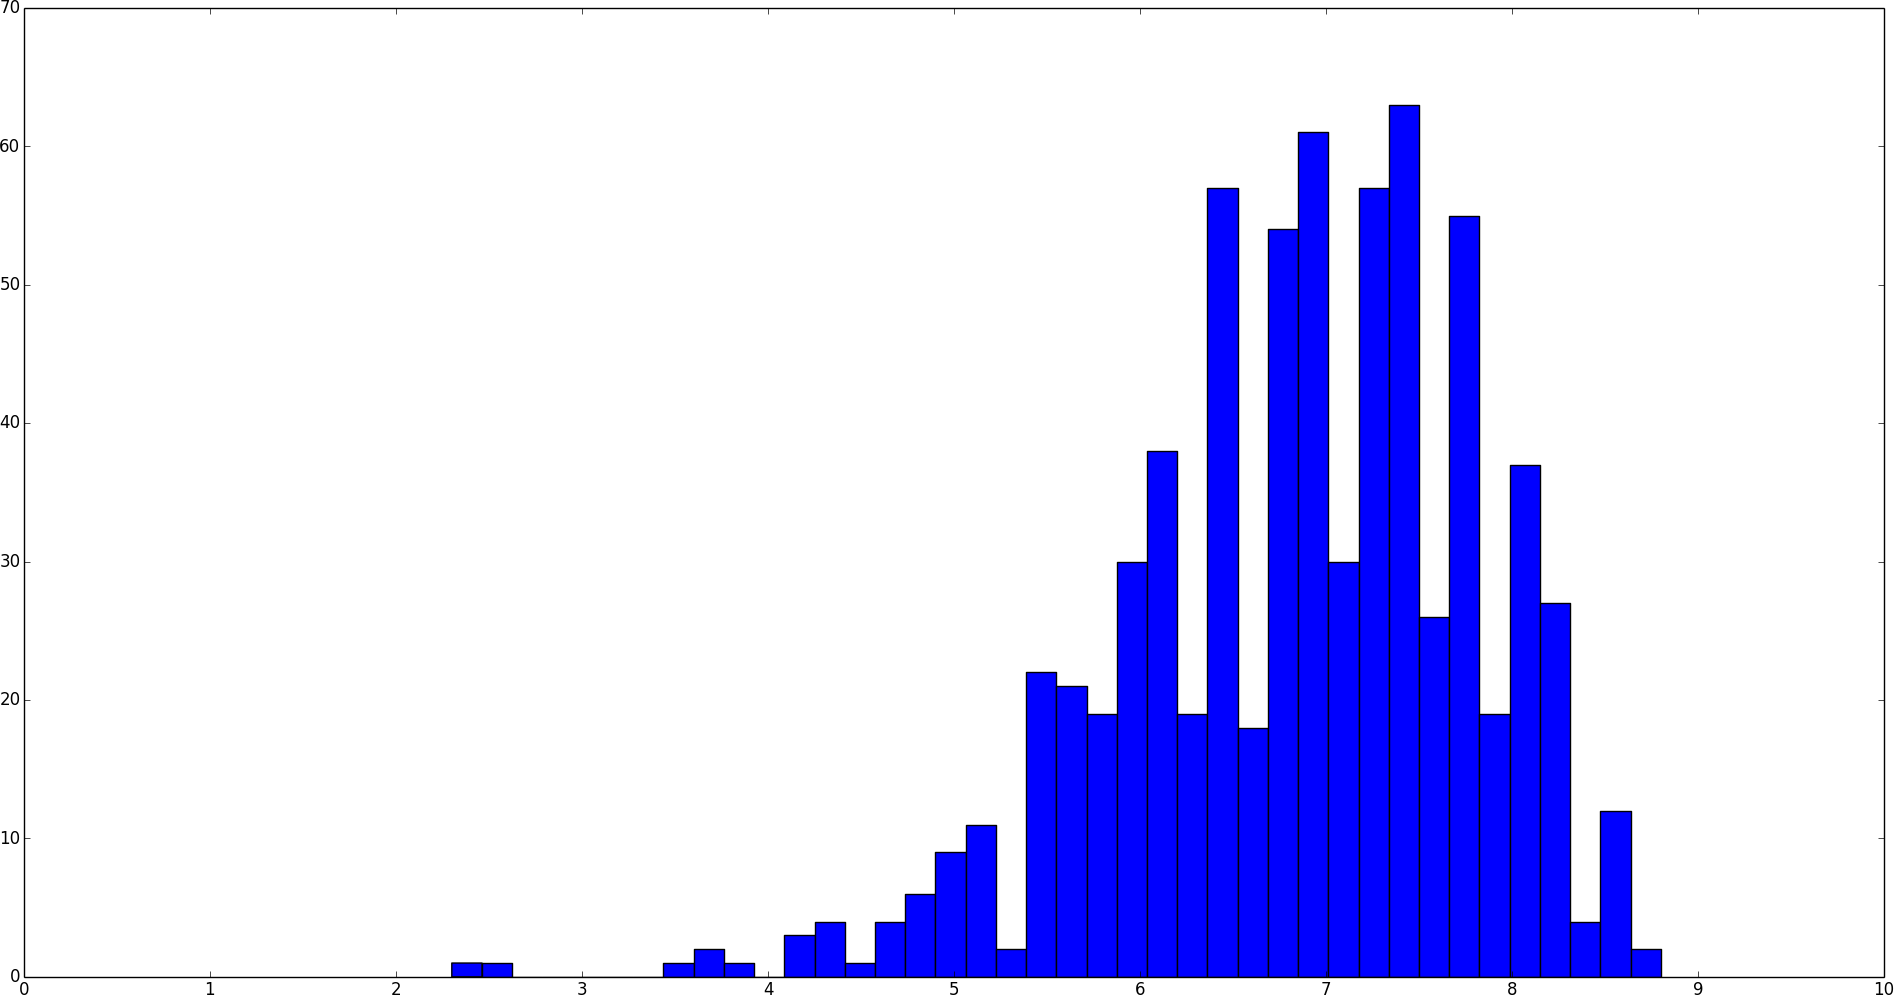
\includegraphics[width=\textwidth]{scores_histogram.png}
  \caption{Score distribution between 0 and 10 of the complete data set.}
  \label{fig:scorehist}
\end{figure}

Notice how almost all scores lie between 6 and 8.
This is likely due to the fact that the scripts on IMSDb are requested and provided by users of the website. 
So a movie that is liked by many people will have a high chance to have its script being requested and supplied on IMSDb.
This results in this skewed distribution: a movie on IMSDb will have a high chance to be liked by many people.

Another thing to note is that IMDb uses a weighted average, instead of the arithmetic average for its score.
According to IMDb, `various filters are applied to the raw data in order to eliminate and reduce attempts at ``vote stuffing'' by individuals more interested in changing the current rating of a movie than giving their true opinion of it.''
The exact formula that is used to calculate the weighted average is kept secret, to be able to maintain its effectiveness. 

This weighted average can vary quite significantly with the arithmetic mean. 
For example, the arithmatic mean of the scores of the movie ``The Amityville Asylum'' is 3.3, while its weighted average is 2.6.
IMDb claims the weighted score provides a more accurate vote average than the arithmatic mean.

\section{Approach}
\label{sec:approach}
%• Explain the model; if any important assumptions are made at this stage, explain why they are reasonable or necessary
%• Explain learning / inference algorithms
In this section we explain our model, and show the derivations we use for the Gibbs sampler.

\subsection{Model}
In this section we describe the extended topic based model we used.
It is taken from \cite{SLDA}.

The generative version of LDA is as follows:
\begin{enumerate}
  \item Draw topic proportions $\theta \mid \alpha \sim \Dir(\alpha)$.
  \item For each word:
  \begin{enumerate}
    \item Draw topic assignment $z_n \mid \theta \sim \Mult(\theta)$.
    \item Draw word $w_n \mid z_n, \beta_{1:K} \sim \Mult(\beta_{zn})$.
  \end{enumerate}
\end{enumerate}
Its graphical representation can be seen in Figure~\ref{fig:LDA}.
It makes use of the hyperparameters $\alpha$, which influences the topic distributions of a document, and of $\beta$, which influences the topic definitions of each topic.

\begin{figure}[ht!]
  \centering
  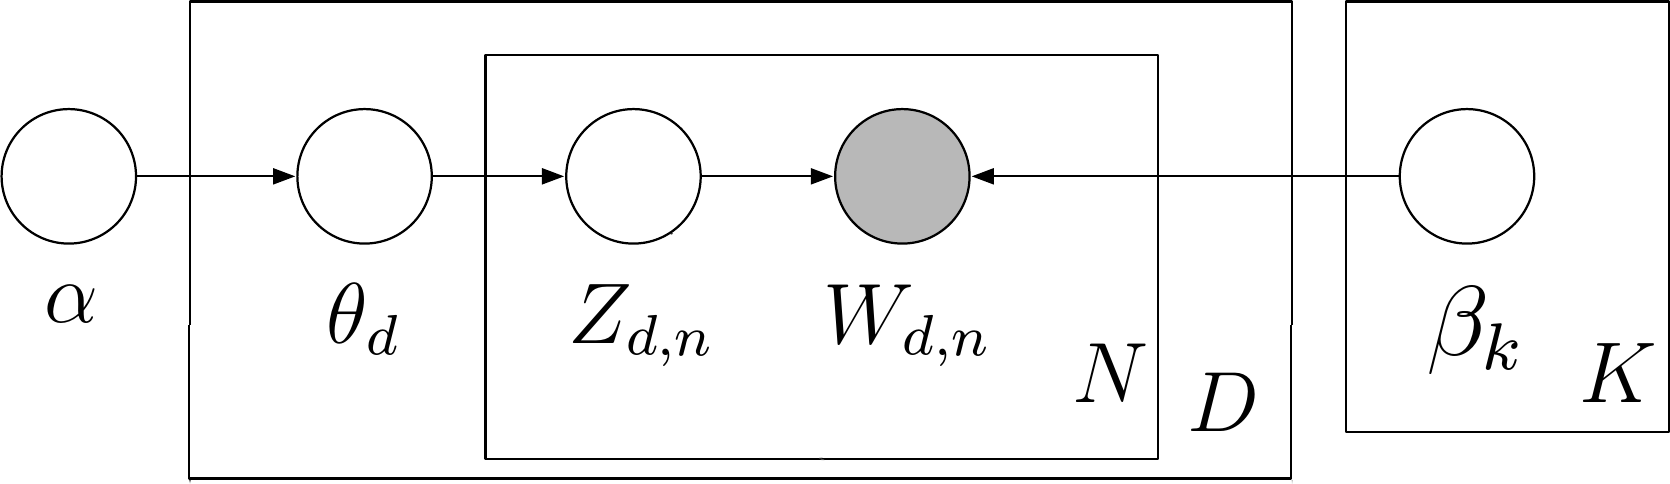
\includegraphics[width=0.6\textwidth]{LDA.png}
  \caption{A graphical representation of traditional LDA model.}
  \label{fig:LDA}
\end{figure}

We however, use an extended version of LDA, which makes use of the given scores. 
Because of this, a third step is added to the generative process:

\begin{enumerate}
  \item Draw topic proportions $\theta \mid \alpha \sim \Dir(\alpha)$.
  \item For each word:
  \begin{enumerate}
    \item Draw topic assignment $z_n \mid \theta \sim \Mult(\theta)$.
    \item Draw word $w_n \mid z_n, \beta_{1:K} \sim \Mult(\beta_{zn})$.
  \end{enumerate}
  \item[3.] Draw response variable $y \mid z_{1:N}, \eta, \sigma^2 \sim \mathcal{N}(\eta^\top \bar{z}, \sigma^2)$.
\end{enumerate}

This version can be called supervised LDA or SLDA.
Its graphical representation can be seen in Figure~\ref{fig:SLDA}.
Note that we use a symmetric $\alpha$ and $\beta$, i.e. $\alpha=(\alpha_1, \alpha_2, \dots, \alpha_K)$, where $\forall i,j \leq K: \alpha_i = \alpha_j$ and similar for $\beta$.

\begin{figure}[ht!]
  \centering
  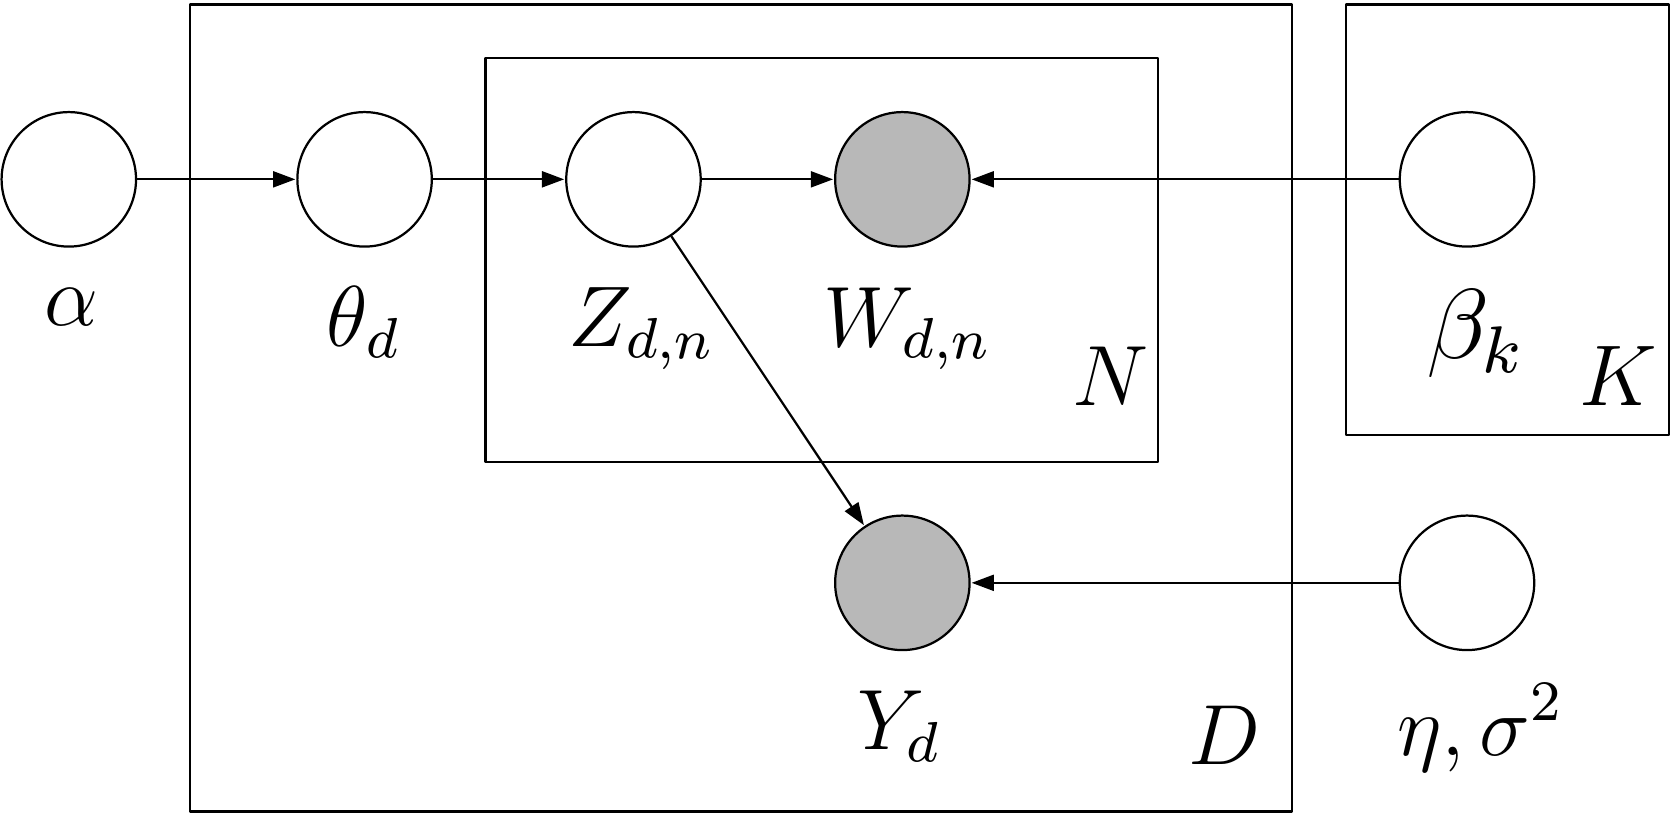
\includegraphics[width=0.6\textwidth]{SLDA.png}
  \caption{A graphical representation of our modified LDA model.}
  \label{fig:SLDA}
\end{figure}

\subsubsection{Collapsed Supervised Latent Dirichlet Allocation}
In this section we will give the derivations for the collapsed supervised LDA model.

We start by recalling the full likelihood expression (i.e. for all variables, both latent and visible) of the model:
\begin{equation}
\label{eq:prodpart}
\begin{gathered}
P(\Phi, \Theta, S, Z, W \mid \alpha, \beta, \eta, \sigma) = \left[ \prod_{k = 1}^K \Dir(\phi_k \mid \beta) \right]  \\
\times \left[ \prod_{d = 1}^D \Dir(\theta_d \mid \alpha) \mathcal{N}(s_d \mid \eta^\top \bar{z}_d, \sigma) \prod_{i = 1}^{N_d} \Mult(z_{di} \mid \theta_d) \Mult(w_{di} \mid \varphi_{z_{di}}) \right]
\end{gathered}
\end{equation}

The final collapsed SLDA will only give probabilities for \(S, Z\) and \(W\). 
To achieve this, we will first integrate out the latent variable $\Phi$. The first thing that can be noticed is that every $\varphi_k$ is independently sampled, and thus can be integrated separately:
\begin{equation}
P(\Theta, S, Z, W \mid \alpha, \beta, \eta, \sigma) = \int_{\phi_0}\int_{\phi_1}\cdots \int_{\phi_K} P(\Phi, \Theta, S, Z, W \mid \alpha, \beta, \eta, \sigma)
\end{equation}
At this point we need to rewrite part of Equation~\ref{eq:prodpart} in order to be able to continue the derivation:
\begin{equation}
\prod_{d = 1}^D \prod_{i = 1}^{N_d} \Mult(w_{di} \mid \phi_{z_{di}}) = \prod_{d = 1}^D \prod_{w = 1}^W \prod_{k = 1}^K \Mult(w \mid \phi_k)^{N_{dk}},
\end{equation}
where $N_d$ represents the total number of words within document $d$, and $N_{dk}$ represents the number of words within document $d$ assigned to topic $k$.
\begin{equation}
\begin{gathered}
P(\Theta, S, Z, W \mid \alpha, \beta, \eta, \sigma) = \left[ \prod_{k = 1}^K \int_{\phi_k} \Dir(\phi_k \mid \beta) \prod_{d = 1}^D \prod_{w = 1}^W \Mult(w \mid \phi_k)^{N_{dk}} \right]  \\
\times\left[ \prod_{d = 1}^D \Dir(\theta_d \mid \alpha) \mathcal{N}(s_d \mid \eta^\top \bar{z}_d, \sigma) \prod_{i = 1}^{N_d} \Mult(z_{d, i} \mid \theta_d) \right]
\end{gathered}
\end{equation}
We can now make use of the definition of the Dirichlet-Multinomial distribution in order to solve all the integrals:
\begin{equation}
\begin{gathered}
P(\Theta, S, Z, W \mid \alpha, \beta, \eta, \sigma) = \left[ \prod_{k = 1}^K \frac{ \Gamma(W\beta)}{\Gamma(N_k + W\beta)} \prod_{w = 1}^W \frac{\Gamma(N_{kw}+\beta)}{\Gamma(\beta)}\right]\\
\times\left[ \prod_{d = 1}^D \Dir(\theta_d \mid \alpha) \mathcal{N}(s_d \mid \eta^\top \bar{z}_d, \sigma) \prod_{i = 1}^{N_d} \Mult(z_{di} \mid \theta_d) \right]
\end{gathered}
\end{equation}
We can proceed in an analogous fashion in order to integrate out the latent $\Theta$ parameter:
\begin{equation}
P(S, Z, W \mid \alpha, \beta, \eta, \sigma) = \int_{\theta_0}\int_{\theta_1}\dots \int_{\theta_D} p(\Theta, S, Z, W \mid \alpha, \beta, \eta, \sigma)
\end{equation}
This gives us:
\begin{equation}
\begin{gathered}
P(S, Z, W \mid \alpha, \beta, \eta, \sigma) =  \left[ \prod_{k = 1}^K \frac{ \Gamma(W\beta)}{\Gamma(N_k + W\beta)} \prod_{w = 1}^W \frac{\Gamma(N_{kw}+\beta)}{\Gamma(\beta)}\right]  \\
\times\left[ \prod_{d = 1}^D \mathcal{N}(s_d \mid \eta^\top \bar{z}_d, \sigma) \frac{\Gamma(K\alpha)}{\Gamma(N_d + K \alpha)} \prod_{k = 1}^K \frac{\Gamma(N_{dk} + \alpha)}{\Gamma(\alpha)} \right]
\end{gathered}
\end{equation}
Note that $\Gamma(\beta)$ and $\Gamma(\alpha)$ are constant in these products, so they can be moved outside of the product.
\begin{equation}
\begin{gathered}
P(S, Z, W \mid \alpha, \beta, \eta, \sigma) = \left[ \prod_{k = 1}^K \frac{ \Gamma(W\beta)}{\Gamma(\beta)^W \Gamma(N_k + W\beta)} \prod_{w = 1}^W \Gamma(N_{kw}+\beta)\right]\\
\times\left[ \prod_{d = 1}^D \mathcal{N}(s_d \mid \eta^\top \bar{z}_d, \sigma) \frac{\Gamma(K\alpha)}{\Gamma(\alpha)^K \Gamma(N_d + K \alpha)} \prod_{k = 1}^K \Gamma(N_{dk} + \alpha) \right]
\end{gathered}
\end{equation}

\subsubsection{Collapsed Gibbs Sampler}

Using Bayes' theorem, we know that:

\begin{equation}
P(Z \mid S, W, \dots) = \frac{P(S, W \mid Z, \dots) P(Z \mid \dots)}{P(S, W \mid \dots)} \propto P(S, W, Z \mid \dots),
\end{equation}
where we did not write all model hyperparameters for the sake of clarity.
Thus, in order to implement a Gibbs sampler for this model, we have that:
\[P(z_{di} = k \mid Z^{\backslash{i}}, S, W, \alpha, \beta, \eta, \sigma) \propto P(z_{di} = k, Z^{\backslash{i}}, S, W, \alpha, \beta, \eta, \sigma) = \]
\[  \left[ \prod_{k' = 1}^K \frac{ \Gamma(W\beta)}{\Gamma(\beta)^W \Gamma(N_k'^{\backslash i} + \mathbb{I}(k' = k) + W\beta)} \prod_{w = 1}^W \Gamma(N_{k'w}^{\backslash i} + \mathbb{I}(k' = k \wedge w = w_{di}) + \beta)\right] \]
\[ \times\left[ \prod_{d = 1}^D \mathcal{N}\left(s_d\, \left| \vphantom{\frac{1}{1}} \right. \, \eta^T \frac{N_{d{k'}}^{\backslash i} + \mathbb{I}(k' = k)}{N_d}, \sigma \right) \frac{\Gamma(K\alpha)}{\Gamma(\alpha)^K \Gamma(N_d^{\backslash i} + K \alpha)} \prod_{k' = 1}^K \Gamma(N_{dk'}^{\backslash i} + \mathbb{I}(k' = k) + \alpha) \right] \]

Where we used $ \frac{N_{dk}}{N_d} \equiv \bar{z_d} $ and $\mathbb{I}(condition) = 1$ iff the condition evaluates to true, and zero otherwise. We can further simplify the previous expression by removing those factors that are constant across all possible values for $k$, resulting in the following final collapsed Gibbs sampler:
\begin{equation}
\begin{gathered}
P(z_{di} = k \mid Z^{\backslash{i}}, S, W, \dots) \propto \left[ \prod_{k'} \frac{\prod_w \Gamma(N_{{k'}w}^{\backslash i} + \mathbb{I}(k' = k \wedge w = w_{di}) + \beta)}{\Gamma(N_{k'}^{\backslash i} + \mathbb{I}(k' = k) + W \beta)} \right]  \\
\times \mathcal{N}\left(s_d\, \left| \vphantom{\frac{1}{1}} \right. \, \eta^T \frac{N_{d{k'}}^{\backslash i} + \mathbb{I}(k' = k)}{N_d}, \sigma \right) \prod_{k'} \Gamma(N_{d{k'}}^{\backslash i} + \mathbb{I}(k' = k) + \alpha),
\end{gathered}
\end{equation}

The Gibbs sampler can also be expressed in log-space probabilities, in order to get a more numerically-stable implementation:
\begin{equation*}
\begin{gathered}
\log P(z_{di} = k \mid Z^{\backslash{i}}, S, W, \alpha, \beta, \eta, \sigma)\\
\begin{aligned}
&\propto\sum_{k',w} \left[ \log \Gamma(N_{{k'}w}^{\backslash i} + \mathbb{I}(k' = k \wedge w = w_{di}) + \beta) - \log \Gamma(N_{k'}^{\backslash i} + \mathbb{I}(k' = k) + W \beta) \right]\\
&-\frac{1}{2 \sigma^2}\left(s_d - \eta^\top \frac{N_{d{k'}}^{\backslash i} + \mathbb{I}(k' = k)}{N_d}\right)^2 + \sum_{k'} \log \Gamma(N_{d{k'}}^{\backslash i} + \mathbb{I}(k' = k) + \alpha)
\end{aligned}
\end{gathered}
\end{equation*}

\subsubsection{Rewriting the log-gamma function}
The logarithm of the gamma function can be rewritten as follows \cite{BorosMoll}:
\begin{equation}
  \log \Gamma(z) = -\gamma z - \log z + \sum_{j=1}^\infty \left[\frac{z}{j}-\log\left(1+\frac{z}{j}\right)\right],
\end{equation}
where $\gamma$ is the Euler-Mascheroni constant. 
We apply this to $\sum_k \sum_w \log \Gamma(N_{kw} + \beta)$, which then becomes:
\begin{align*}
&=\sum_{k, w} -\gamma (N_{kw} + \beta) -\log (N_{kw} + \beta) + \sum_{j=1}^\infty \frac{N_{kw} +\beta}{j}-\log\left(1 + \frac{N_{kw} + \beta}{j}\right)\\
&=-\gamma (N + KW\beta) - \sum_{k,w} \log (N_{kw}+\beta) - \sum_{j=1}^\infty  \frac{N_{kw} + \beta}{j} - \log\left(\frac{N_{kw} + \beta+j}{j}\right)\\
\intertext{
Note that the term \(-\gamma (N + KW\beta)\) serves as a normalisation constant for this dataset.
Since we do not need the exact probabilities but only the proportional probabilities during the algorithms execution, we can discard those terms.
}
&\Rightarrow - \sum_{k,w} \log (N_{kw}+\beta) - \sum_{j=1}^\infty  \frac{N_{kw} + \beta}{j} - \log\left(\frac{N_{kw} + \beta+j}{j}\right)\\
&=-\sum_{k,w} \log (N_{kw}+\beta) - \sum_{j=1}^\infty  \frac{N_{kw} + \beta}{j} - \log(N_{kw} + \beta+j) + \log(j)\\
&=-\sum_{k,w} \log (N_{kw}+\beta) - \sum_{j=1}^\infty \left( \frac{N_{kw} + \beta}{j} +\log(j)\right) + \sum_{j=1}^\infty \log(N_{kw} + \beta + j)\\
&=\sum_{j=1}^\infty \left( \frac{N + KW\beta}{j} +KW\log(j)\right) - \sum_{k,w} \log (N_{kw}+\beta) + \sum_{j=1}^\infty \log(N_{kw} + \beta + j)\\
&=\sum_{j=1}^\infty \left( \frac{N + KW\beta}{j} +KW\log(j)\right) - \sum_{k,w} \sum_{j=0}^\infty \log(N_{kw} + \beta + j)
\end{align*}

Again, the term \(\sum_{j=1}^\infty  \frac{N + KW\beta}{j} +KW\log(j)\) is a constant for this dataset, so we can discard it.
This results in the following proportionality:
\begin{align}
  \sum_{k,w} \log \Gamma(N_{kw} + \beta) &\propto  -\sum_{k,w}\sum_{j=0}^\infty \log (N_{kw} + \beta + j)
\intertext{Using similar steps, we can also simplify}
  \sum_k \log\Gamma (N_k + W\beta) &\propto -\sum_k \sum_{j=0}^\infty \log(N_k + W\beta + j)\\
  \sum_{k,d} \log \Gamma(N_{dk} + \alpha) &\propto -\sum_{k,d} \sum_{j=0}^\infty \log(N_{dk}+\alpha +j)\\
  \sum_d \log \Gamma (N_d + K\alpha) &\propto -\sum_d \sum_{j=0}^\infty \log(N_d + K\alpha + j)
\end{align}

Putting these together gives us the following proportionality:
\begin{equation*}
\begin{gathered}
\log P(z_{di} = k \mid Z^{\backslash{i}}, S, W, \alpha, \beta, \eta, \sigma) \\
\begin{aligned}
&\propto \sum_{j=0}^\infty \sum_{k'}\log(N_{k'}^{\backslash i} + \mathbb{I}(k' = k) + W \beta + j) -\log(N_{d{k'}}^{\backslash i} + \mathbb{I}(k' = k) + \alpha +j)\\
&-\sum_{j=0}^\infty \sum_{k',w} \log(N_{{k'}w}^{\backslash i} + \mathbb{I}(k' = k \wedge w = w_{di}) + \beta + j) -\frac{1}{2 \sigma^2}\left(s_d - \eta^\top \frac{N_{d{k'}}^{\backslash i} + \mathbb{I}(k' = k)}{N_d}\right)^2
\end{aligned}
\end{gathered}
\end{equation*}

In practice, however, we can not calculate the infinite terms of the above sums, and thus we would stop the approximation at some arbitrary iteration $J$:

\[ \log P(z_{di} = k \mid Z^{\backslash{i}}, S, W, \alpha, \beta, \eta, \sigma) \]
\[ \propto -\frac{1}{2 \sigma^2}\left(s_d - \eta^\top \frac{N_{d{k'}}^{\backslash i} + \mathbb{I}(k' = k)}{N_d}\right)^2 + \sum_{k'} \sum_{j=0}^J \log(N_{k'}^{\backslash i} + \mathbb{I}(k' = k) + W \beta + j) \]
\[ -\log(N_{d{k'}}^{\backslash i} + \mathbb{I}(k' = k) + \alpha +j) + \sum_{w} \log(N_{{k'}w}^{\backslash i} + \mathbb{I}(k' = k \wedge w = w_{di}) + \beta + j) \]

\subsubsection{Estimating response parameters}
The maximum a posteriori (MAP) estimate for the hyperparameter \(\eta\)  can be inferred from the gradient of the complete model likelihood:
\begin{equation}
\nabla_{\eta_k} \log P(S, Z, W \mid \alpha, \beta, \eta, \sigma) = \sum_d \frac{1}{\sigma^2} \frac{N_{dk}}{N_d} \left( s_d - \eta^T \frac{N_{d\cdot}}{N_d}\right)
\end{equation}
\[= \sum_d \frac{s_d \frac{N_{dk}}{N_d} }{\sigma^2} - \sum_d \frac{ \frac{N_{dk}}{N_d} \left( \eta^T \frac{N_{d\cdot}}{N_d} \right) }{\sigma^2}\]

For the MAP estimate, the gradient should be zero.
This allows us to rewrite the above formula into:
\begin{align*}
\sum_d s_d \frac{N_{dk}}{N_d} &= \sum_d \frac{N_{dk}}{N_d} \left( \sum_{k'} \eta_{k'} \frac{N_{dk'}}{N_d} \right)\\
\sum_d s_d \frac{N_{dk}}{N_d} &= \sum_d \frac{N_{dk}}{N_d} \left( \eta_k \frac{N_{dk}}{N_d} + \sum_{k' \ne k} \eta_{k'} \frac{N_{dk'}}{N_d} \right) \\
\sum_d s_d \frac{N_{dk}}{N_d} &= \eta_k \sum_d \left( \frac{N_{dk}}{N_d}  \right)^2 + \sum_d \left( \frac{N_{dk}}{N_d} \sum_{k' \ne k} \eta_{k'} \frac{N_{dk'}}{N_d} \right) \\
\intertext{Further rewriting finally gives us the MAP estimate for \(\eta\):}
\eta_k \sum_d \left( \frac{N_{dk}}{N_d}  \right)^2  &=\sum_d \left( s_d \frac{N_{dk}}{N_d} - \frac{N_{dk}}{N_d} \sum_{k' \ne k} \eta_{k'} \frac{N_{dk'}}{N_d} \right)\\
\eta_k \sum_d \left( \frac{N_{dk}}{N_d}  \right)^2 &=  \sum_d \frac{N_{dk}}{N_d} \left( s_d - \sum_{k' \ne k} \eta_{k'} \frac{N_{dk'}}{N_d} \right)\\
\eta_k &= \frac{\sum_d \frac{N_{dk}}{N_d} \left( s_d - \sum_{k' \ne k} \eta_{k'} \frac{N_{dk'}}{N_d} \right)}{\sum_d \left( \frac{N_{dk}}{N_d}  \right)^2} \numberthis \label{eq:etaupdate}
\end{align*}
From our experiments, we noticed that trying to apply the formula as described in Equation~\ref{eq:etaupdate} as an update rule for \(\eta\) does not converge.
Instead, the following update can be used:
\begin{equation}
\eta_k^{new} \leftarrow (1 - \gamma) \eta_k^{old} + \gamma \frac{\sum_d \frac{N_{dk}}{N_d} \left( s_d - \sum_{k' \ne k} \eta_{k'} \frac{N_{dk'}}{N_d} \right)}{\sum_d \left( \frac{N_{dk}}{N_d}  \right)^2 + \epsilon},
\end{equation}
where we used $1 \gg \gamma > 0$ in order for the previous series to converge and $1 \gg \epsilon > 0$ as a smoothing constant.

\section{Experiments}
\label{sec:experiments}
%• Any details about experiments (dataset sizes, parameter selection, etc)
%• Results
%• Analysis (discussion of results / visualization / findings / etc)

For our experiments we chose to use two different performance measures: perplexity and inverse accuracy.

\subsection{Perplexity}

The perplexity measure is commonly used within LDA literature, and we include it for reference purposes. 
It is defined as follows:
\begin{equation}
\text{Perplexity} \equiv \exp \left\{ -\frac{1}{N} \sum_{i = 1}^N \log P(x_i)  \right\},
\end{equation}
where \(P(x_i)\) represents the probability the model gives for the $i$-th item within the test set. The lower the perplexity, the less ``surprised'' the model is of seeing its input, which indicates a better model.

This measure has a shortcoming, though. 
It is enough for the model to give a probability of zero to a word to drive this performance measure to infinity. 
This does not mean, however, that the model is infinitely bad, since the rest of the items might still have large probabilities.
To overcome this problem, we also measure the performance in terms of the average inverse accuracy of the model.

\subsection{Inverse accuracy}

The average inverse accuracy of the model is defined as follows:
\begin{equation}
\text{Accuracy}^{-1} \equiv \frac{1}{\frac{1}{N}\sum_{i = 1}^N P(x_i)}
\end{equation}
This measure should be interpreted as the number of words the model incorrectly predicts for each correctly predicted word. 
The lower this magnitude, the better the model.

\subsection{Results}

We created a first experiment in order to check the validity of our approximation for the Gibbs sampler of our model. 
We selected different values for $J$ and compared the predictive performance for each case. 
We ran three different MCMC chains and then averaged the results. 
Within each execution, 100 movies were randomly selected as the training set, and 20 as the testing set. 
We used 5 samples, taken every 4 steps of the Gibbs sampler, with the first 20 iterations discarded as the burn-in period. 
Our findings are summarized in Table~\ref{table:J}:

\begin{table}[ht!]
\caption{Experiment results for varying values of $J$ with 100/20 movies as training/test set.}
\label{table:J}
\begin{center}
\begin{tabular}{r|cccccc}
J               & 1 & 2 & 3 & 4 & 5 & 6 \\ \hline
Perplexity      & 4100 & 4125 & 4082 & 4251 & 3754 & 3881 \\
Accuracy$^{-1}$ & 858 & 871 & 823 & 863 & 877 & 815 \\
\end{tabular}
\end{center}
\end{table}

We can observe that the predictive performance tends to improve with larger values of $J$. 
This is to be expected, since the higher $J$ is, the better the approximation of the log-gamma function becomes.
This improvement is not, however, very consistent even when averaging across 3 chains, and thus we theorize that the extra computational time spent on making $J$ higher is better used if $J$ is kept as low as possible and more movies and/or iterations are used instead.
We then conclude this approximation is interesting, at least from a computational perspective.

We devised a second experiment in order to find out good values for the number of topics to use in our models.
Again we did an equivalent set up to the one for the previous experiment, but this time changing the number of topics and whether or not the Gibbs sampler uses the movie score information.

\begin{table}[ht!]
\captionsetup{justification=centering}
\caption{Experiment results for varying values of $K$,\\ with $J=1$ and 100/20 movies as training/test set.} 
\label{tab:K}
\begin{center}
\begin{tabular}{c|cc|ccc}

Metric &	LDA topics      & & 25 & 50 & 100 \\ \hline
\multirow{2}{*}{Perplexity} &	\multirow{2}{*}{Using scores?} & No  & 4128 & 5333 & 6954 \\
			  &             & Yes & \textbf{4005} & 5503 & 7082 \\ \hline
\multirow{2}{*}{Accuracy$^{-1}$} & \multirow{2}{*}{Using scores?} & No  & 845 & 1318 & 2049 \\
			      &          & Yes & \textbf{805} & 1372 & 2067 \\
\end{tabular}
\end{center}
\end{table}

We can see how all models start overfitting with, at least, more than 25 topics.
This is most likely due to the fact that we only used 100 movie plot summaries for training, which is a rather small dataset. 
We also observe that, for 25 topics, not only the best predictive performance is achieved, but this is further improved by using the movie scores.
This improvement is very small, but we could systematically observe it in all the tests we run for this work. 

We also wondered which words were the most correlated with either bad or good movie scores. In order to discover this, the hyperparameter $\eta$ can be multiplied with the topic definitions $\Phi$, and the resulting vector ordered by values. Table \ref{table:word_scores} shows a list with the 30 words with the highest positive correlation with movie scores.

\begin{table}[ht!]
\captionsetup{justification=centering}
\caption{Caption here.}
\label{table:word_scores}
\begin{center}
\begin{tabular}{c|c}
Word (after stemmer) & Score \\ \hline
his & 2.86 \\
he & 2.34 \\
(empty) & 1.64 \\
her & 1.48 \\
who & 1.14 \\
she & 0.882 \\
they & 0.870 \\
their & 0.843 \\
him & 0.795 \\
has & 0.788 \\
be & 0.766 \\
when & 0.750 \\
from & 0.749 \\
find & 0.541 \\
one & 0.516 \\
get & 0.500 \\
up & 0.471 \\
have & 0.466 \\
life & 0.461 \\
out & 0.449 \\
after & 0.444 \\
man & 0.406 \\
take & 0.401 \\
this & 0.388 \\
new & 0.357 \\
becom & 0.356 \\
world & 0.351 \\
into & 0.346 \\
time & 0.346 \\
them & 0.329 \\
\end{tabular}
\end{center}
\end{table}

\section{Discussion}
\label{sec:discussion}
%• Refer to the research questions you defined in your introduction.
%• Any related work you are aware of?
%• Challenges you observed?
%• “Future work” (you do not need to do this work really J, but what would you change in the model / what experiments you would run / etc, if you would have a chance to do this? What other people should look into?
%• Any thoughts / observation / wider implications

Discussion

\subsubsection*{Acknowledgments}
%Use unnumbered third level headings for the acknowledgments. 
%All acknowledgments go at the end of the paper.
%Do not include acknowledgments in the anonymized submission, only in the final paper. 

Acknowledgments

\vspace*{-3\baselineskip}
\renewcommand{\refname}{\subsubsection*{References}} % Using "References" as the title of the bibliography section
% \vspace*{-1em}
\begin{thebibliography}{9}
\bibitem{SLDA}
  David M. Blei, Jon D. McAuliffe;
  \emph{Supervised Topic Models};
  Neural Information Processing Systems 21 (2007)
  
\bibitem{IMDb}
  IMDb.com, Inc.; 
  \emph{IMDb, the world's most popular and authorative source for movie, TV and celebrity content};
  \url{www.imdb.com}
  
\bibitem{IMSDb}
  IMSDB.com; 
  \emph{Internet Movie Script Database - Movie scripts free for reading and downloading};
  \url{www.imdsb.com}

\bibitem{MovieRegression}
  M. Joshi, D. Das, K. Gimpel, N. A. Smith;
  \emph{Movie Reviews and Revenues: An Experiment in Text Regression};
  In Proceedings of NAACL-HLT (2010)

\bibitem{PredictStars}
  A. T. Scaria, R. M. philip, S. V. Mehta;
  \emph{Predicting Star Ratings of Movie Review Comments};\\
  \url{http://cs229.stanford.edu/proj2011/MehtaPhilipScaria-Predicting\%20Star\%20Ratings\%20from\%20Movie\%20Review\%20Comments.pdf}
  
\bibitem{lingua}
  Jim Richardson, Benjamin Franz;
  \emph{Lingua Stem};
  Freerun Technologies, Inc; (1999);
  \url{http://search.cpan.org/~snowhare/Lingua-Stem-0.84/lib/Lingua/Stem.pod}

\bibitem{BorosMoll}
  Geogre Boros, Victor H. Moll,
  \emph{Irresistible Integrals: symbolics, analysis and experiments in the evaluation of integrals};
  Cambridge University Press (2004)

\end{thebibliography}

\end{document}
